%%%%%%%%%%%%%%%%%%%%%%%%%%%%%%%%%%%%%%%%%%%%%%%%%%%%%%%%%%%%%%%%%%%%%%%%%%%%%%%%%%
% The Ascon state
%
% public domain (CC0 1.0 https://creativecommons.org/publicdomain/zero/1.0/)
%%%%%%%%%%%%%%%%%%%%%%%%%%%%%%%%%%%%%%%%%%%%%%%%%%%%%%%%%%%%%%%%%%%%%%%%%%%%%%%%%%

\documentclass[10pt]{standalone}

\newif\ifsans
\newif\iftext
\newif\ifhorizontal
\newif\ifvertical
\newif\ifcolor
\horizontalfalse
\verticalfalse

%%% CONFIGURATION %%%%%%%%%%%%%%%%%%%%%%%%%%%%%%%%%%%%%%%%%%%%%%%%%%%%%%%%%%%%%%%%
\sanstrue   % for sans-serif fonts (slides, web)
%\sansfalse % for serif fonts (article)

\texttrue   % include phase description
%\textfalse % no phase description

\colortrue   % use color for highlights
%\colorfalse % no color

%\horizontaltrue % highlight horizontal word
%\verticaltrue % highlight vertical slice
%%%%%%%%%%%%%%%%%%%%%%%%%%%%%%%%%%%%%%%%%%%%%%%%%%%%%%%%%%%%%%%%%%%%%%%%%%%%%%%%%%

\ifsans
\usepackage[default,tabular]{sourcesanspro}
\usepackage{sfmath}
\fi

\usepackage{tikz}
\usetikzlibrary{shadows}
\ifcolor
  \definecolor{webred}{HTML}{663333}
\else
  \definecolor{webred}{HTML}{444444}
\fi

\begin{document}
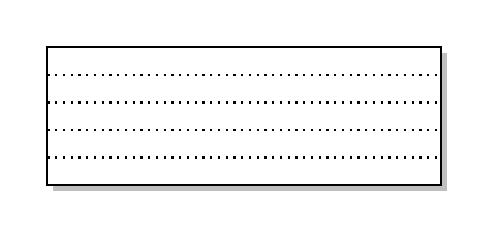
\begin{tikzpicture}[thick, scale=0.5]
  \draw[fill=white, drop shadow] (0,0) rectangle (10,3.5);
  \draw[dotted] (0,.7) -- (10,.7)
                (0,1.4) -- (10,1.4)
                (0,2.1) -- (10,2.1)
                (0,2.8) -- (10,2.8);
  \iftext
    \draw (9,.35) node {$S_4$}
         ++(0,.7) node {$S_3$}
         ++(0,.7) node {$S_2$}
         ++(0,.7) node {$S_1$}
         ++(0,.7) node {$S_0$};
  \fi

  \ifhorizontal
    \draw[color=webred,fill=white,drop shadow={shadow yshift=-.7ex}] (-.3,2.05) rectangle +(10.6,.9);
    \draw (9.2,2.5) node {$S_1$};
  \fi
  \ifvertical
    \draw[color=webred,fill=white,drop shadow={shadow xshift=.7ex}] (2.5,-.3) rectangle +(.7,4.1);
  \fi

  \path (-.5,-.5) rectangle (10.5,4.0); % phantom
\end{tikzpicture}
\end{document}
